\section*{Abstract}

This thesis explores the design and implementation of a \acrfull*{dt} for a green smart home, integrating \acrfull*{eud} with \acrfull*{ml} algorithms.\@ \acrshort*{eud} approaches enable users to control and manage their \acrfull*{iot} environments, e.g.\ using trigger-action routines~\parencite{barricelliEnduserDevelopmentEnduser2019}. This work is significant because automatic behaviors like routines may have potential to develop effective energy management systems for homes. Furthermore, \acrshort*{dt}s are already successfully used for modeling and optimizing complex systems
in various domains.

The \acrshort*{dt} developed in this thesis enhances energy consumption awareness by allowing users to monitor the energy consumption of smart appliances throghout the day and simulate scenarios related to the creation of routines. These simulations assess the effects of the activation of appliances involved in the routines and potentially modify them to save energy based on the \acrshort*{dt}'s suggestions. The \acrshort*{dt} is implemented as a \acrfull*{rest} \acrfull*{api} that exposes endpoints for accessing and manipulating the data and routines of the smart home, displaying the energy consumption of the appliances over time, and simulating the effects of adding new routines and resolving potential conflicts with the existing ones. The \acrshort*{api} separates the \acrshort*{dt} logic from the user interface, enabling the \acrshort*{dt} to be integrated with various clients. A web frontend was also developed to showcase the functionalities of the \acrshort*{dt}. The functionality of the \acrshort{dt} is based on a list of appliances in the home with the supported operation modes (e.g., washing modes for a washing machine, or on/off for a lamp), along with a set of routines which activate the appliances to certain operation modes at specific times during the day.

An hypothetical home was designed as a starting point for the creation of the \acrshort*{dt}, containing appliances extracted from the GREEND\footnote{\url{https://www.andreatonello.com/greend-energy-metering-data-set/}}~\parencite{monacchiGREENDEnergyConsumption2014} and UK-DALE\footnote{\url{https://jack-kelly.com/data/}}~\parencite{kellyUKDALEDatasetDomestic2015} power consumption datasets. These datasets were selected through a scoping review among power consumption datasets available in the literature, because of the large number of appliances gathered in European households they provide. This is important to minimize geographic variations in appliance usage patterns and to produce results that are relevant for Italian households. The selected datasets however do not record the operation mode of appliances. For example, a washing machine could be in a certain wash program at a given time, which has a specific duration and energy requirement. This information is required to assign a specific energy consumption value to the operation modes and to estimate their duration.

This limitation is overcome with an approach inspired by~\cite{castangiaClusteringApplianceOperation2023}, which suggests using unsupervised deep learning techniques to cluster appliance operation modes from a learned, latent state representation of the raw data. Figure~\ref{fig:high-level-procedure} illustrates the main steps of the approach. First, a segmentation procedure is applied to the raw appliance data to identify the active states that contain the actual power signatures of the device. These signatures are then standardized and fed to a deep autoencoder model, which learns to reconstruct the operation cycles and encode them into a latent representation. Next, a K-means clustering algorithm is applied to the
latent representation, to group the operation cycles into different programs of the device. Finally, the clusters are mapped to the operation modes of the appliance.

\begin{figure}
    \centering
    
\includegraphics[width=.9\linewidth]{images/high_level_procedure.png}
    \caption{High level procedure for identifying the operation modes of appliances}%
    \label{fig:high-level-procedure}
\end{figure}

The \acrshort*{dt} uses the identified operation modes and the user-defined routines to create a state matrix of the smart home throughout the day. Figure~\ref{fig:state-matrix} shows an example of a state matrix, displaying the operation modes of the appliances in the hypothetical home throughout the day, based on a predefined set of routines. When a user wants to create a new routine to manage their appliances, the \acrshort*{dt} allows them to simulate what would happen in case of its activation, by returning different types of feedback associated with different scenarios. The state matrix makes it straightforward to simulate the addition of a new automation and check if any previously mentioned scenarios occur. The process starts by creating a copy of the current state matrix and by updating it with the new appliance states of the automation under creation. During simulation, the following conflict scenarios may happen:
\begin{itemize}
    \item \textit{The power consumption exceeds the energy meter load capacity}: the routine can not be executed because it includes an appliance activation that will bring the total energy consumption over the maximum load capacity for the energy meter (in Italy it is commonly set to 3kWH for domestic use). The \acrshort*{dt} provides suggestions on how the automation could be modified. For example, its activation could be postponed after an appliance involved in another automation has completed its operation;
    \item \textit{Inconsist operation modes}: the automation under creation includes the activation of an appliance in a given operation mode (e.g., for a washing machine, a short sports cycle), but there is another automation scheduled on the same appliance with a different operation mode in an overlapping time slot. The DT may present the user with different options: the deletion of one of the two conflicting automations or the modification of one of them;
    \item \textit{No conflict, but a suggestion to be more sustainable}: the \acrshort{dt} may suggest reducing energy consumption costs, avoiding cases of non-sustainable appliance activation. The \acrshort{dt} also looks for the best activation time slot for the automation, taking into account the energy cost of starting the automation at every minute of the day
\end{itemize}

\begin{figure}
    \centering
    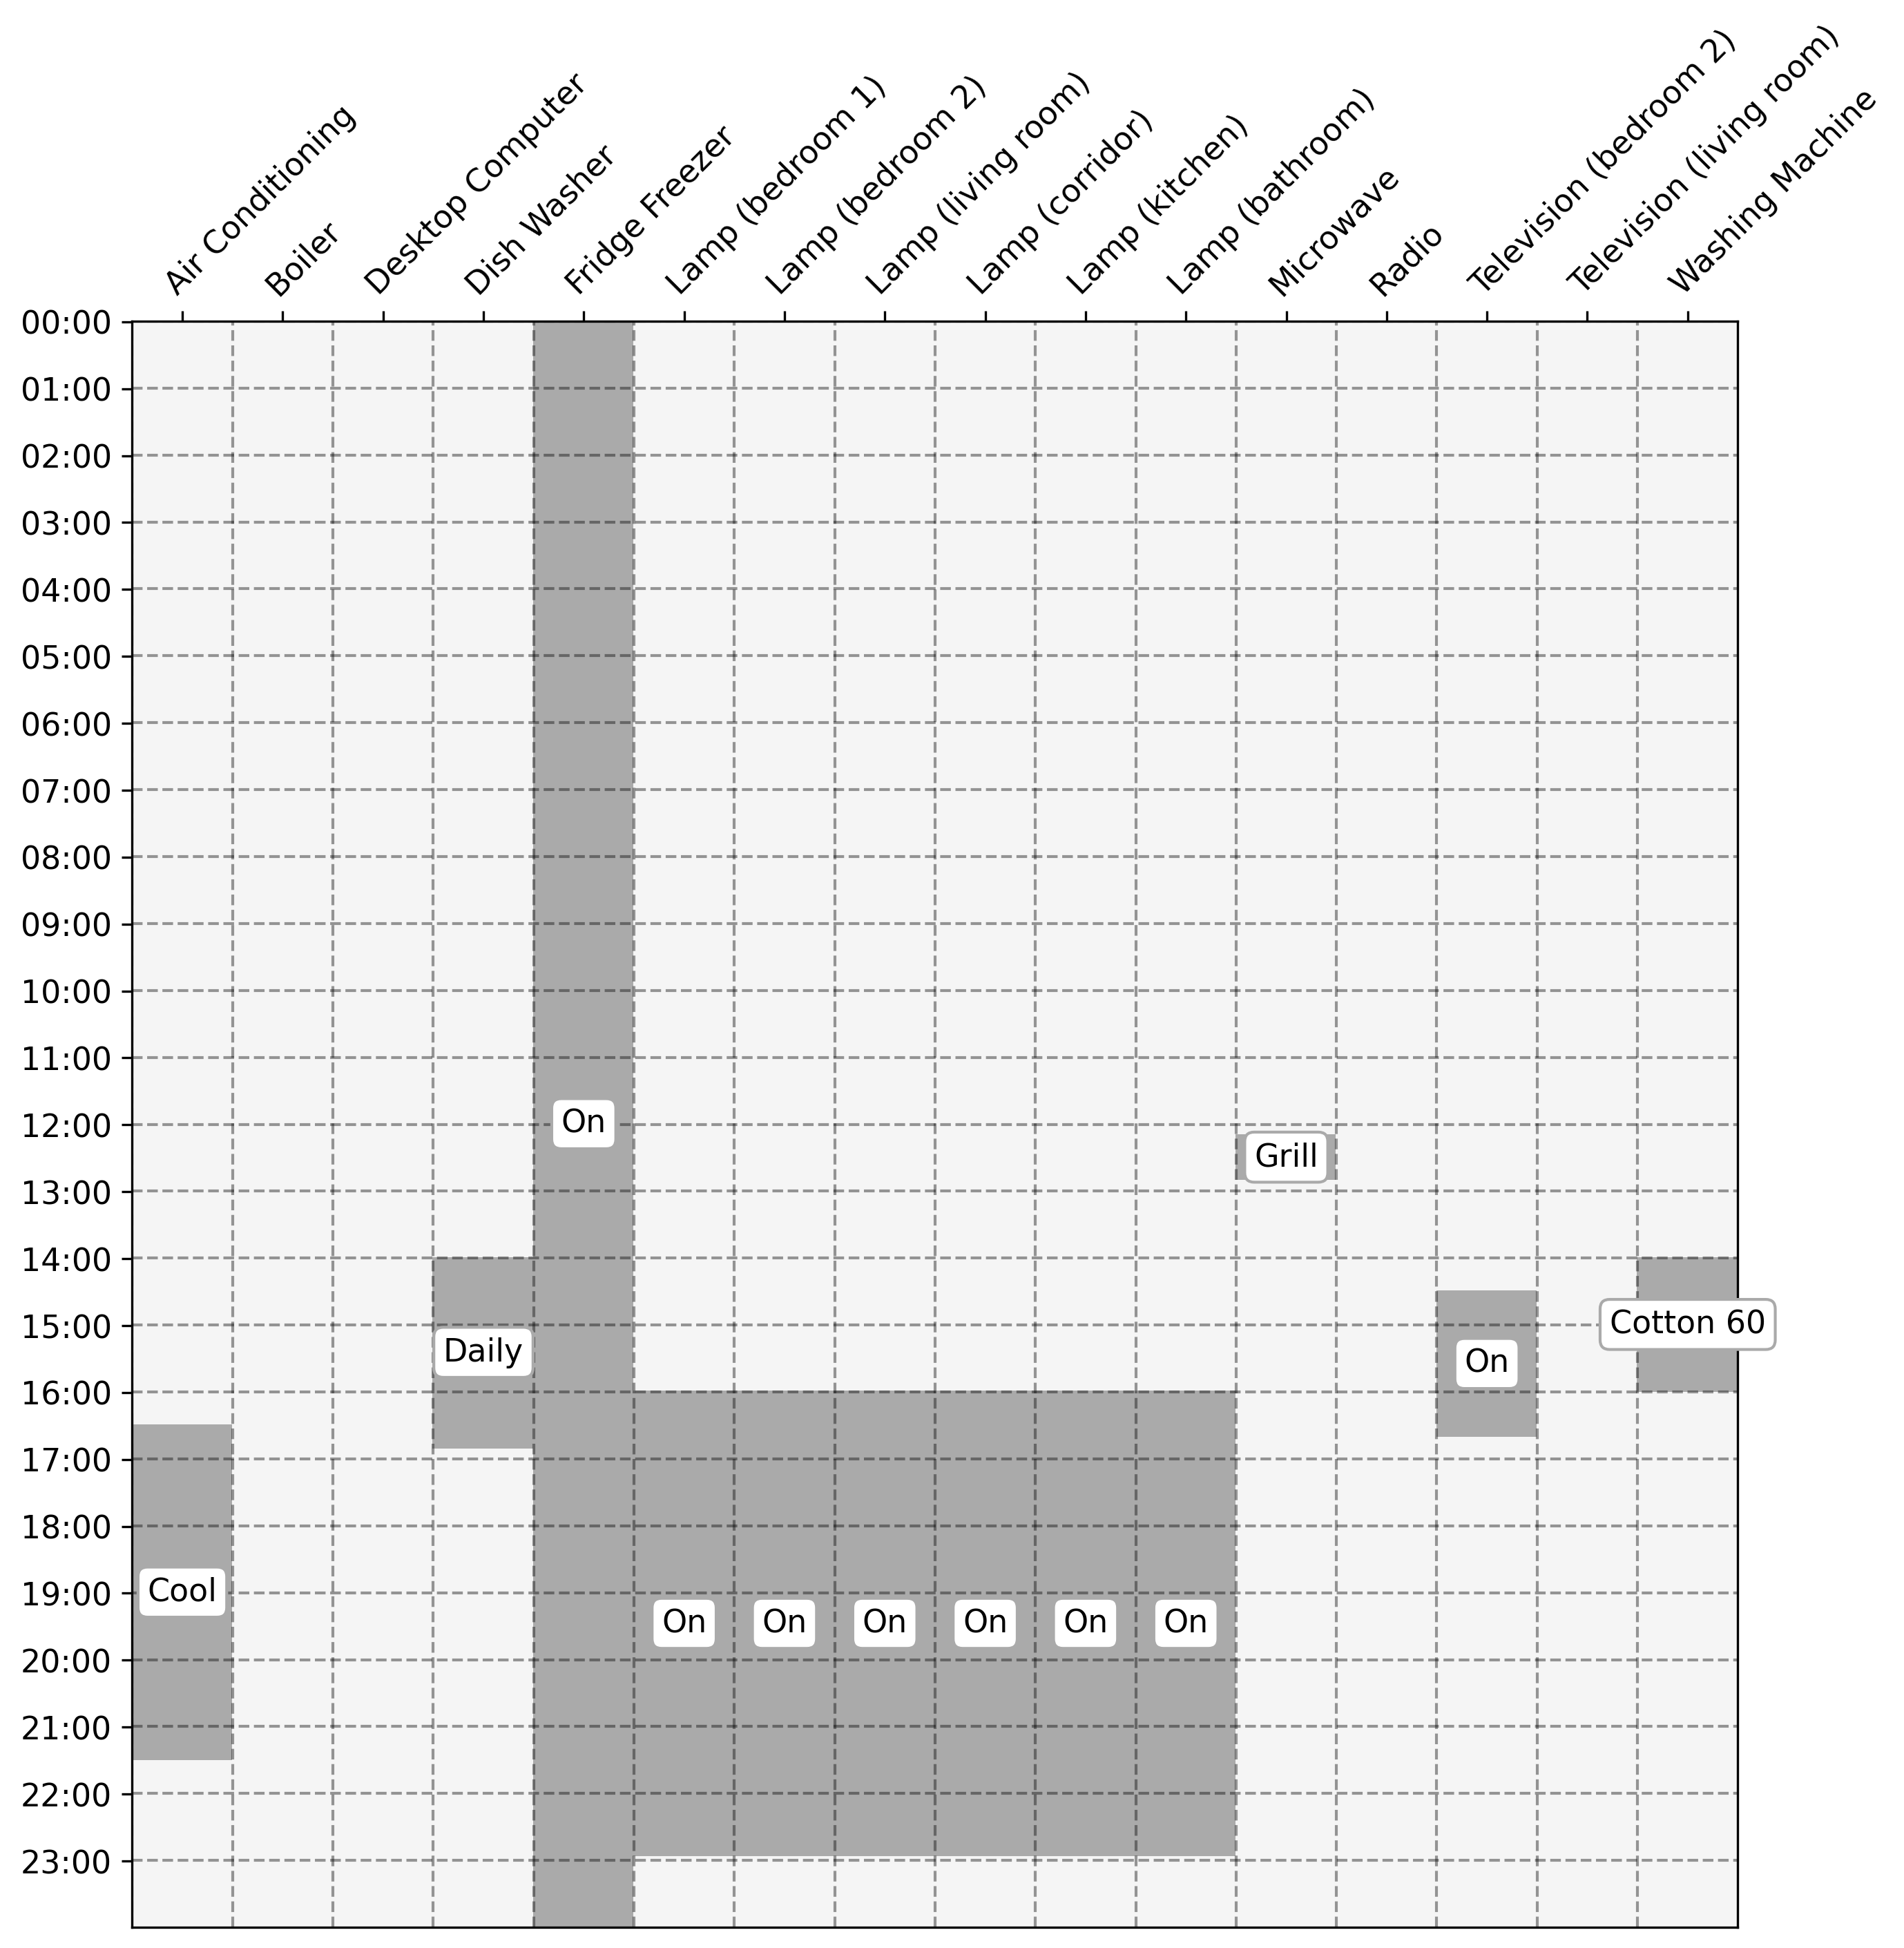
\includegraphics[width=.55\linewidth]{images/real_matrix.png}
    \caption{Example of a state matrix}%
    \label{fig:state-matrix}
\end{figure}

This research is significant as it contributes to the development of a new paradigm for smart and sustainable living, and advances both theoretical and practical knowledge of \acrshort*{dt}s in the building sector.